\chapter{Execute Stage}

\section{Execute}

In the last lab, you created the ALU and ALU Control modules.  Now we will finish the iExecute stage by creating a new module called iExecute.  The iExecute module should consist of everything shown in the red box in Figure ~\ref{fig:execute_stage}.  To implement the iExecute stage, you will need to create iExecute.v and add the following components to it:
 
\begin{enumerate}
	\item ALU module from the previous lab
	\item ALU Control module from the previous lab	
	\item Mux to select the source of the second input into the ALU.  You can reuse your mux that you created in the iFetch stage.
	\item Shifter to left shift the sign extended branch address offset.  You should NOT create a new module for this.  Instead, you should add code directly in iExecute.v since the left shift can be accomplished with a single line of code. 
	\item Adder to add the branch address offset to the current PC.  You can reuse your adder that you created in the iFetch stage.  Please note the adder is near the top of the datapath diagram and it has an output named ALU result on the diagram.  In fact, this is not a full ALU, but just an adder.  And our output signal will be named branch\_target, as this is what it really is (rather than naming it ALU\_Result).
\end{enumerate} 

\begin{figure}
	\caption{Execute Stage}\label{fig:execute_stage}
	\begin{center}
		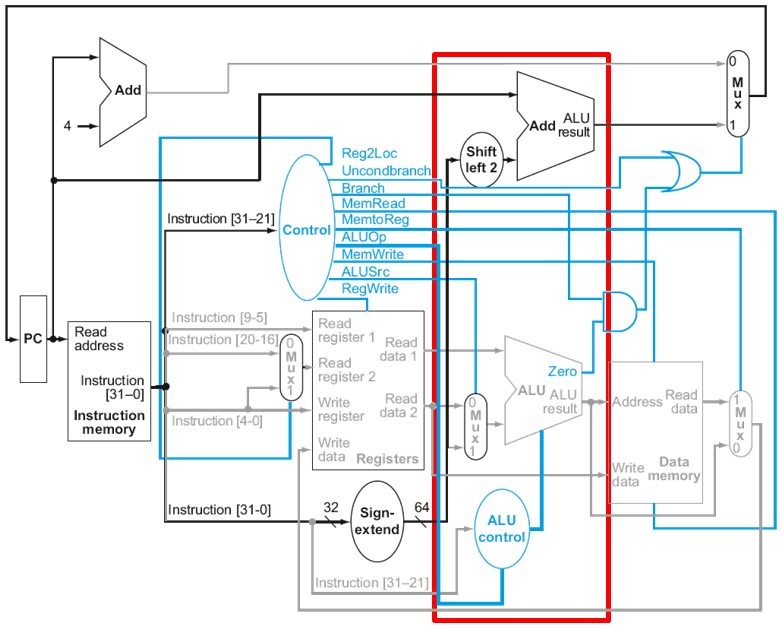
\includegraphics[width=4.75in]{../images/execute_stage.png}
	\end{center}
\end{figure} 


The testbench will run the 10 instructions in your Expected Results Table.  Therefore, your next step is to update your Expected Results Table by updating the 3 outputs of the iExecute stage. You also need to update 1 input to the table, PC.  The PC value should start at 0 and increment by 4 for each instruction.  Populate the iExecute output rows with expected values for each instruction.  All of the inputs that you need to determine the expected result are in the table.  Make sure to use N/A if the signal is not applicable for a given instruction.

Finally, you need to complete the testbench.  I have provided the bulk of the testbench.  The only updates that you need to make to the testbench are:
\begin{enumerate}
	\item I have X for all er values right now.  Please update these to the correct values per your Expected Results Table.
	\item I have a verify function call for all 3 outputs for every instruction.  If an output is N/A for a particular instruction, remove or comment out that verify.  There should be a total of 20 test cases.  
\end{enumerate}   


\section{Integrating Fetch, Decode, and Execute}
We now have working Fetch, Decode, and Execute modules.  Now it is time to put them together to produce a system that can:
\begin{enumerate}
	\item Update the program counter
	\item Read the appropriate instruction from the instruction datafile
	\item Read the correct registers
	\item Update all control lines
	\item Sign extend address data
	\item Calculate Branch Target Addresses
	\item Provide a zero bit for conditional branch instructions
	\item Produce ALU results for R-Type and D-Type instructions
\end{enumerate}

Once we can do all of this, we will be ready for the iMemory stage.  We currently have the fetch and decode module integrated into fd\_integration.sv.  We also have a working execute module.  Today we need to integrate the execute module with the fetch and decode stages.  The new testbench should be called fde\_integration.sv.  Please reuse the instructions from your Expected Results Table that you used when you integrated fetch and decode.  Once integrated, you should be able to produce a simulation that includes the outputs of fetch and decode as well as 3 new outputs from execute:
\begin{enumerate}
	\item Branch Target
	\item ALU Result
	\item Zero
\end{enumerate}   

These three new outputs are marked on Figure Figure ~\ref{fig:integrated_execute}.  To verify these outputs, you should have already  updated the Expected Results Table to include these three outputs.  To test this integration, I recommend copying the contents of fd\_integration.sv into fde\_integration.sv and then modifying from there, adding your execute module, cr values, verify statements, etc that are necessary to verify the integration of the execute module. fd\_integration had 139 test cases, so fde\_integration should have 159 test cases.

\begin{figure}
	\caption{Execute Stage}\label{fig:integrated_execute}
	\begin{center}
		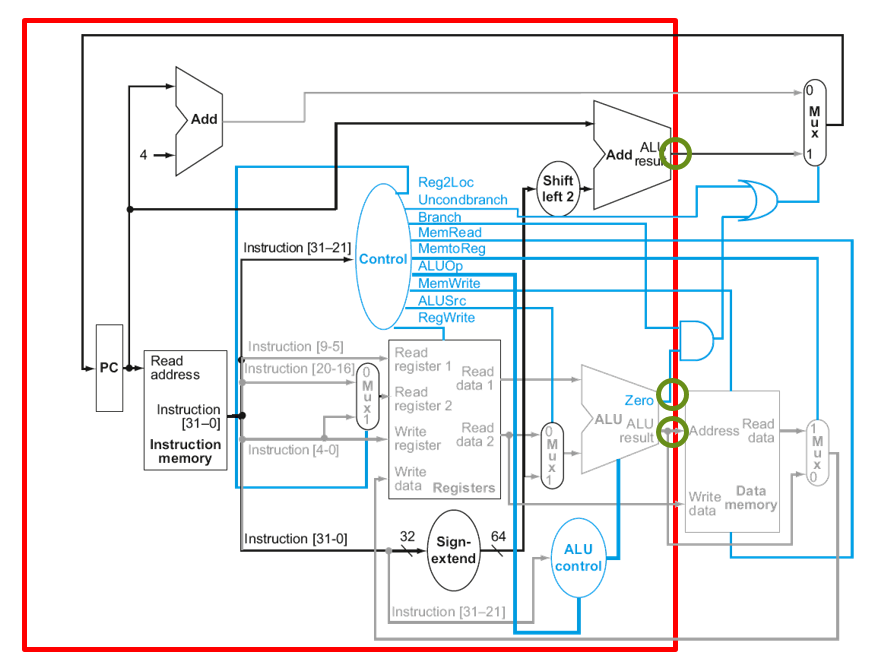
\includegraphics[width=4.75in]{../images/integrated_execute.png}
	\end{center}
\end{figure} 

\section{Your Assignment}
You are to:
\begin{enumerate}
\item Complete the iExecute module 
\item Update your Expected Results Table with the outputs from the iExecute stage.  Also add a PC value if it is not in the table yet. 
\item Update iExecute\_test.sv
\item Verify that your simulation results match your expected results.
\item Create fde\_integration.sv
\item Verify that your simulation results match your expected results.
\item Rather than writing a lab report, please produce a landscape mode PDF file called Lab9\_lastname.pdf that includes (in this order):
\begin{enumerate}
	\item Your name and the lab number.
	\item A snip of your completed Expected Results Table.
	\item A snip of the Simulation Results for the iExecute test and fde\_integration test.  Please show instructions in hex, opcodes and control signals in binary and everything else in signed decimal.  
	\item Copy and paste the entire log from BEGIN TEST RESULTS to END TEST RESULTS into your file.  The results have gotten too long to use the snipping tool.	
\end{enumerate}
\item Upload Lab9\_lastname.pdf file to Canvas.
\item Zip up your ARM-Lab directory and submit it on Canvas as well.  Please make sure that you give me the ARM-Lab directory rather than the ARM-Project directory.  I do not want the project files in the ARM-Project directory.  Before you submit your zip file, extract the file and make sure that the top-level directory is called ARM-Lab and that the lower level directories like code, manual, etc are directly beneath ARM-Lab in the directory structure.  I will extract your zip file and run your code against my correct testbench to verify that your code and testbench work correctly, and it is critical that everyone's directory structure is consistent.
\end{enumerate} 